% Time-budget ablation: judge score by time limit and derailment level
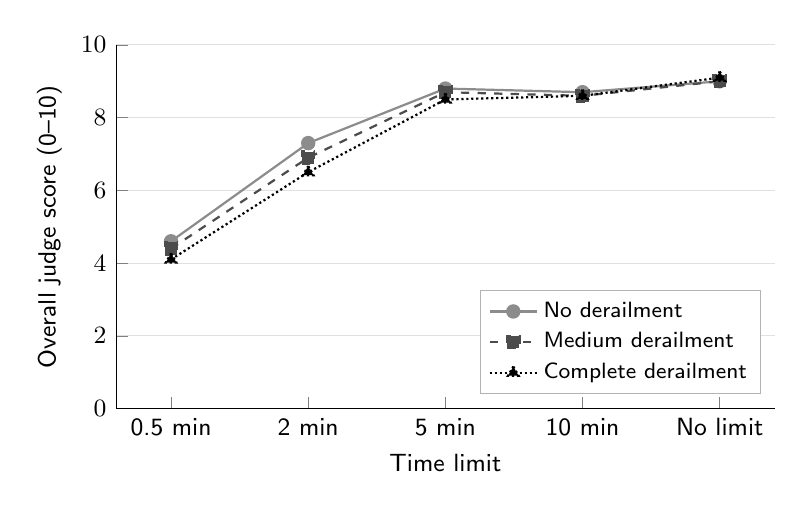
\begin{tikzpicture}
\begin{axis}[
  width=0.82\linewidth, height=6.2cm,
  font=\sffamily\small,
  symbolic x coords={0.5 min, 2 min, 5 min, 10 min, No limit},
  xtick=data,
  ymin=0, ymax=10, ytick={0,2,4,6,8,10},
  ylabel={Overall judge score (0--10)},
  xlabel={Time limit},
  ymajorgrids, grid style={black!12},
  axis lines*=left,
  legend style={at={(0.98,0.04)}, anchor=south east, font=\sffamily\footnotesize, draw=black!30},
  legend cell align=left,
  every axis plot/.append style={thick, mark size=2.2pt},
]
\addplot[color=black!45, mark=*] coordinates {(0.5 min,4.60) (2 min,7.30) (5 min,8.80) (10 min,8.70) (No limit,9.00)};
\addplot[color=black!70, mark=square*, dashed] coordinates {(0.5 min,4.40) (2 min,6.90) (5 min,8.70) (10 min,8.60) (No limit,9.00)};
\addplot[color=black, mark=triangle*, densely dotted] coordinates {(0.5 min,4.10) (2 min,6.50) (5 min,8.50) (10 min,8.60) (No limit,9.10)};
\legend{No derailment, Medium derailment, Complete derailment}
\end{axis}
\end{tikzpicture}
